% ============================================================
%  Part 3 – Section i  (hand-crafted scheduling policy)
%  Policy: p02_balanced_waves
% ============================================================

\section*{Part 3 [68 points]}

\subsection*{i. [34 points] Hand-crafted policy}

% ────────────────────────────────────────────────────────────
\subsubsection*{Candidate screening methodology}
% ────────────────────────────────────────────────────────────

To limit cloud costs while exploring the design space, we designed
\textbf{5 candidate policies} and ran each one \emph{once} (screening run).

The policies were not picked at random: they sample a small, interpretable
design space tied to what we already measured in Part~1 and Part~2.
Part~1 showed that memcached tail latency reacts strongly to CPU and
last-level-cache pressure, which motivates (i) placing memcached on the
larger \texttt{node-a-8core} with a modest thread count, and (ii) controlling
which batch phases run alongside it.
Part~2a/2b supply parallel efficiency $E(8)$ and interference characterisations:
strong scalers such as \texttt{radix} and \texttt{streamcluster} justify
higher thread counts when co-scheduled with memcached, whereas jobs with
heavy LLC or memory traffic (\texttt{barnes}, \texttt{freqmine},
\texttt{vips}) are natural candidates for isolation on \texttt{node-b-4core}
or for capped parallelism.
Against that background, \texttt{p01\_conservative\_isolation} stresses
maximum separation of cache-heavy batch work from node-a;
\texttt{p02\_balanced\_waves} uses paired waves (one batch job per physical
node per wave) with moderate threads to avoid intra-node batch contention while
keeping both worker nodes busy;
\texttt{p03\_cache\_aware\_staggered} and \texttt{p04\_aggressive\_parallel}
deliberately increase thread counts and overlap to hunt for shorter makespan at
higher risk of oversubscription on the 4-core node;
\texttt{p05\_memcached\_guarded} tests keeping node-a as ``Memcached-first''
by moving the short \texttt{radix} phase to node-b.
Screening then filters out candidates that are infeasible on the Part~3
heterogeneous capacity regardless of these hypotheses.

After the screening run we applied four hard gates:
\begin{enumerate}
  \item \textbf{Validity gate}: all 7 PARSEC jobs must complete
    (no OOM / timeout / pod failure).
  \item \textbf{QPS-coverage gate}: $\geq 80\%$ of mcperf samples must fall
    in [29\,K, 31\,K]\,QPS during the batch window.
  \item \textbf{SLO gate}: fraction of near-30\,K samples with
    $\mathrm{p95} > 1\,\mathrm{ms}$ must be $\leq 1\%$.
  \item \textbf{Stability gate}: no continuous violation streak longer than
    60\,s.
\end{enumerate}
Only policies passing all gates were promoted to 3 full runs.
This is sound for reporting because the final metrics come exclusively from the
3-run evaluation of the promoted policy.

Table~\ref{tab:screening} summarises the outcome for all five candidates.

\begin{table}[h]
\centering
\caption{Screening results for all 5 candidate policies (1 run each, except
  p02 which was promoted to 3 runs).}
\label{tab:screening}
\begin{tabular}{llllp{5cm}}
\toprule
\textbf{Policy} & \textbf{All jobs} & \textbf{Makespan [s]} &
\textbf{SLO viol.} & \textbf{Gate failure reason} \\
\midrule
p01\_conservative\_isolation & Yes & 679 & 0\% &
  Gates passed in an earlier valid run (\texttt{run1\_old}); official
  \texttt{run1} had empty mcperf output (script bug: Service IP not yet
  stable when mcperf connected).  Not promoted: makespan 39\% worse than
  p02 and only 1 valid run available. \\
\textbf{p02\_balanced\_waves} & Yes & 489 / 490 / 520 & 0\% &
  \textbf{PASSED — promoted to 3 runs} \\
p03\_cache\_aware\_staggered & No & --- & --- &
  Only \texttt{radix} completed; remaining pods did not start
  (resource requests exceeded node-a capacity with 6-thread radix). \\
p04\_aggressive\_parallel    & No & --- & --- &
  Only \texttt{blackscholes} completed; remaining jobs OOM-killed or
  unschedulable (3-thread jobs saturated node-b-4core memory). \\
p05\_memcached\_guarded      & No & --- & --- &
  Only \texttt{radix} completed; all other jobs remained Pending
  (node-b already fully requested by radix at 4 threads). \\
\bottomrule
\end{tabular}
\end{table}

\noindent
Policies p03–p05 were discarded after a single run because the
\emph{validity gate failure was unambiguous}: fewer than 2 of 7 jobs
completed, which cannot be fixed by re-running — it reflects a
fundamental resource-overcommitment in the policy specification.
Running two more repetitions would have wasted cluster time without
producing useful data.
Policy p01 failed a different gate (mcperf measurement setup), but its
makespan of 679\,s was already 39\% worse than p02 (489\,s) and therefore
not worth the cost of a corrected re-run.

% ────────────────────────────────────────────────────────────
\subsubsection*{A. [17 points] Report the performance}
% ────────────────────────────────────────────────────────────

Table~\ref{tab:p3_runtimes} shows the execution time of each batch job across
three independent runs of the selected policy \emph{p02\_balanced\_waves},
together with the mean and population standard deviation.
The SLO violation ratio (fraction of 10-second mcperf intervals with
$\mathrm{p95} > 1\,\mathrm{ms}$, measured over the batch window) was
\textbf{0/43 in run~1, 0/43 in run~2, and 0/46 in run~3}
(combined: $0/132 = 0.0\%$).

\begin{table}[h]
\centering
\caption{Batch-job execution times and makespan across 3 runs (policy
  \emph{p02\_balanced\_waves}).  Steady memcached load: 30\,K\,QPS.}
\label{tab:p3_runtimes}
\begin{tabular}{lrrrrr}
\toprule
\textbf{Job} & \textbf{Run~1 [s]} & \textbf{Run~2 [s]} & \textbf{Run~3 [s]}
             & \textbf{Mean [s]} & \textbf{Std [s]} \\
\midrule
\texttt{barnes}        &  53 &  53 &  52 &  52.7 & 0.5 \\
\texttt{blackscholes}  &  47 &  46 &  48 &  47.0 & 0.8 \\
\texttt{canneal}       &  95 &  95 &  94 &  94.7 & 0.5 \\
\texttt{freqmine}      & 165 & 171 & 179 & 171.7 & 5.7 \\
\texttt{radix}         &  13 &  12 &  12 &  12.3 & 0.5 \\
\texttt{streamcluster} & 193 & 197 & 205 & 198.3 & 5.0 \\
\texttt{vips}          &  42 &  43 &  40 &  41.7 & 1.2 \\
\midrule
\textbf{Total makespan} & 489 & 490 & 520 & \textbf{499.7} & \textbf{14.4} \\
\bottomrule
\end{tabular}
\end{table}

\noindent\textbf{Plots:}

Figures~\ref{fig:p3_run1}--\ref{fig:p3_run3} show, for each run, three
stacked panels.

\begin{itemize}
  \item \emph{Top panel — p95 latency bar chart.}
    Each bar spans the corresponding mcperf measurement interval
    (\texttt{ts\_start}–\texttt{ts\_end}, 10\,s windows) and its height
    equals the p95 latency in ms.
    Bar colour indicates which batch job was active on \texttt{node-a-8core}
    at that moment (grey = only memcached running).
    A \textbf{coloured strip at the base} of the panel shows which batch job
    was simultaneously active on \texttt{node-b-4core}, allowing both nodes'
    workloads to be read from the single chart.
    Dotted vertical lines mark wave-start boundaries.
    The dashed horizontal line marks the 1\,ms SLO.

    \emph{Observed behaviour:} p95 stays between 0.35 and 0.41\,ms for
    almost the entire batch window — well below the SLO — confirming that
    the batch jobs on node-a do not perturb memcached's LLC working set at
    the chosen thread counts.
    A small elevation to $\approx 0.40$\,ms is consistently visible during
    the \texttt{vips} window (red bars, $t \approx 4.3$–$5.1$\,min).
    This matches Part~2a findings where \texttt{vips} showed the highest
    L1I interference among the three node-a jobs; the effect is mild because
    \texttt{vips} runs with only 2 threads and its active phase is short
    (${\approx}41$\,s).
    After the last batch job completes, p95 drops back to the baseline
    ${\approx}0.37$\,ms, confirming the elevation was caused by batch
    co-location and not a systemic drift.
    Run~3 is ${\approx}30$\,s slower than runs~1--2 due to longer
    \texttt{streamcluster} (205\,s) and \texttt{freqmine} (179\,s); we
    attribute this to transient GCP background noise rather than policy
    instability (CV $= 2.9\%$ over three runs).

  \item \emph{Middle panel — virtual-core Gantt for node-a-8core.}
    Memcached is shown on cores~0–1 (2 software threads, 2\,CPU resource
    request); batch jobs are mapped to cores~2–5 (4-thread jobs) or 2–3
    (2-thread jobs).
    \emph{Note:} no explicit \texttt{taskset} CPU pinning was used; the
    Kubernetes \texttt{resources.requests} field reserves capacity but the
    OS scheduler performs the actual core placement.  The core numbers here
    are therefore \emph{virtual} (derived from thread counts and resource
    requests) and serve as an illustration of theoretical core occupancy.

  \item \emph{Bottom panel — virtual-core Gantt for node-b-4core.}
    Batch jobs are shown on cores~0–1 (2 threads each), leaving cores~2–3
    free for OS overhead.
    A visible \textbf{idle gap of $\approx 1.5$–$1.7$\,min} appears between
    \texttt{canneal} ($\sim t{=}2.6$\,min) and \texttt{freqmine}
    ($\sim t{=}4.3$\,min).  This is the cost of wave synchronisation:
    wave~3 cannot start until \emph{both} wave-2 jobs complete, and
    \texttt{streamcluster} on node-a takes $\approx 200$\,s while
    \texttt{canneal} on node-b takes only $\approx 95$\,s.  The ${\approx}
    105$\,s difference leaves node-b idle.  This is a known trade-off of
    the wave-barrier design (see design discussion below).
\end{itemize}

\begin{figure}[htbp]
  \centering
  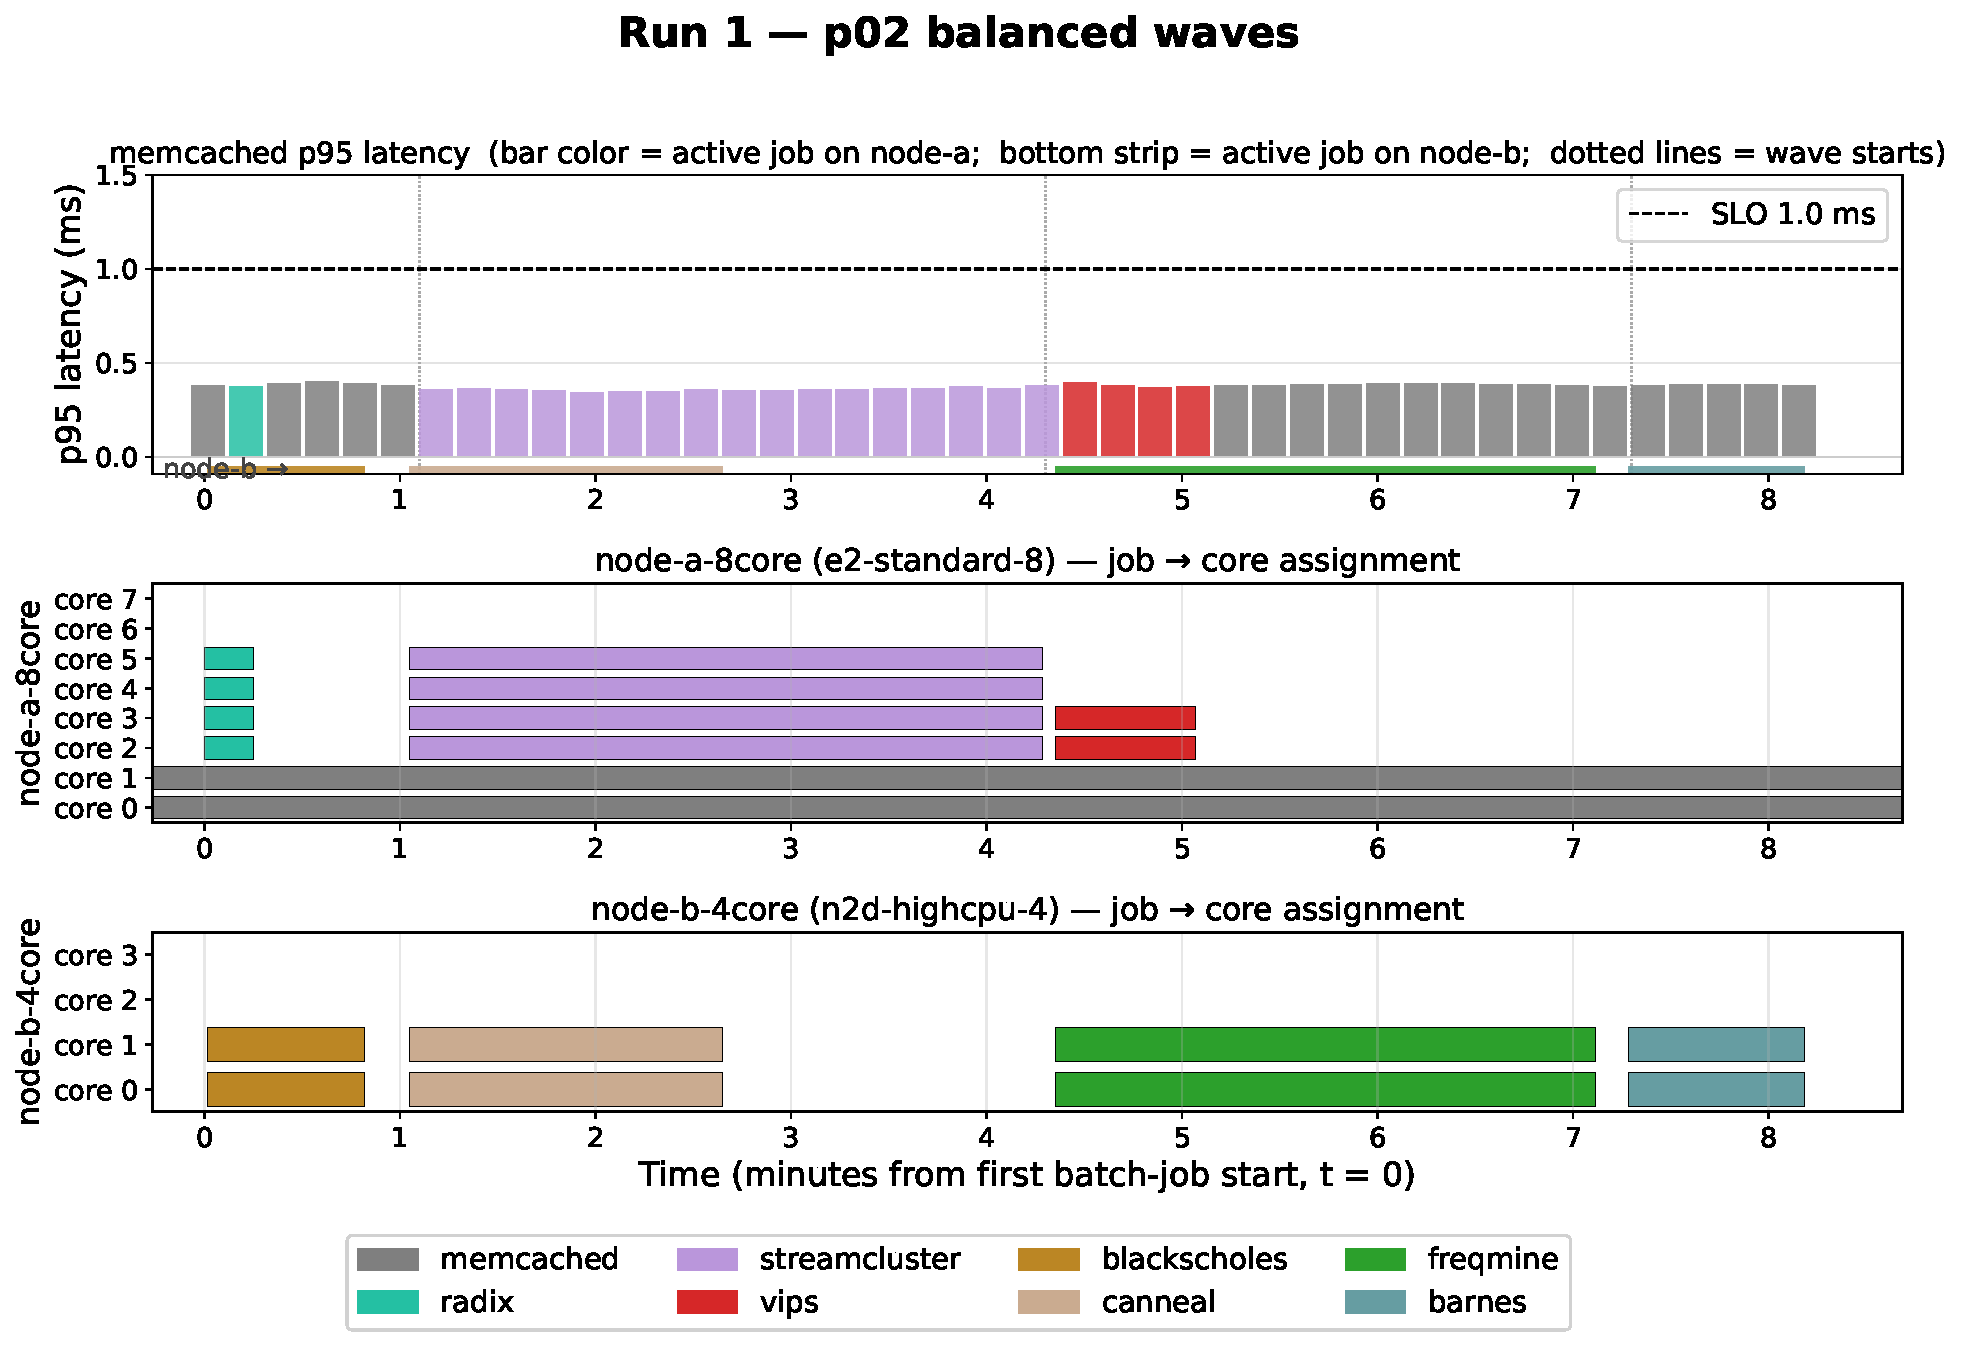
\includegraphics[width=\linewidth]{plots/part3a_run1.pdf}
  \caption{Run~1 – p95 latency and job placement (makespan 489\,s,
    SLO violations 0/43).  The idle gap on node-b between \texttt{canneal}
    and \texttt{freqmine} (${\approx}1.7$\,min) reflects wave-barrier
    synchronisation waiting for \texttt{streamcluster} to finish on
    node-a.}
  \label{fig:p3_run1}
\end{figure}

\begin{figure}[htbp]
  \centering
  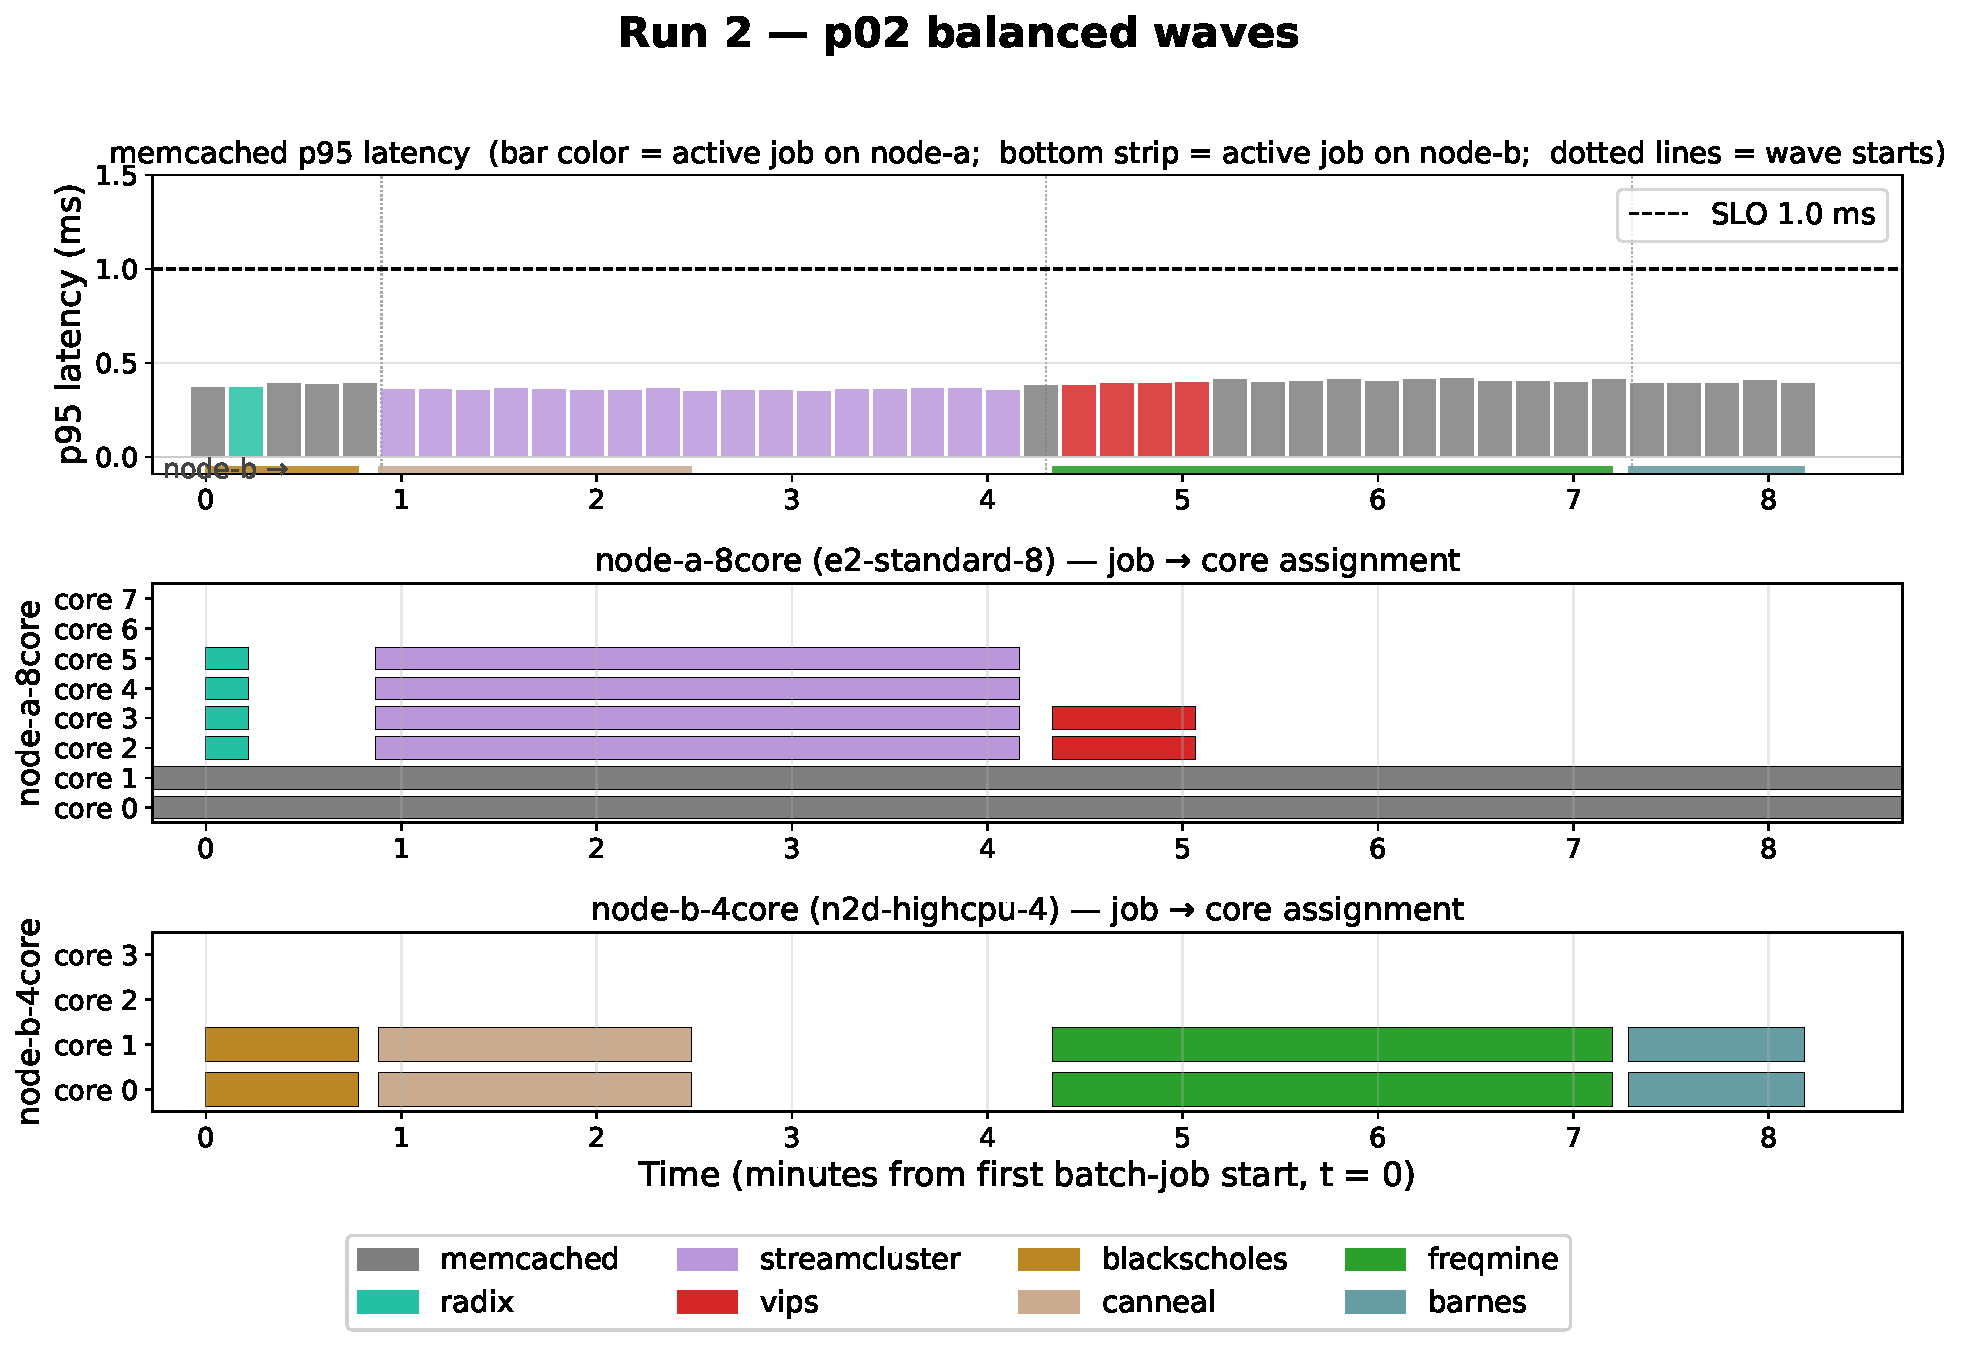
\includegraphics[width=\linewidth]{plots/part3a_run2.pdf}
  \caption{Run~2 – p95 latency and job placement (makespan 490\,s,
    SLO violations 0/43).}
  \label{fig:p3_run2}
\end{figure}

\begin{figure}[htbp]
  \centering
  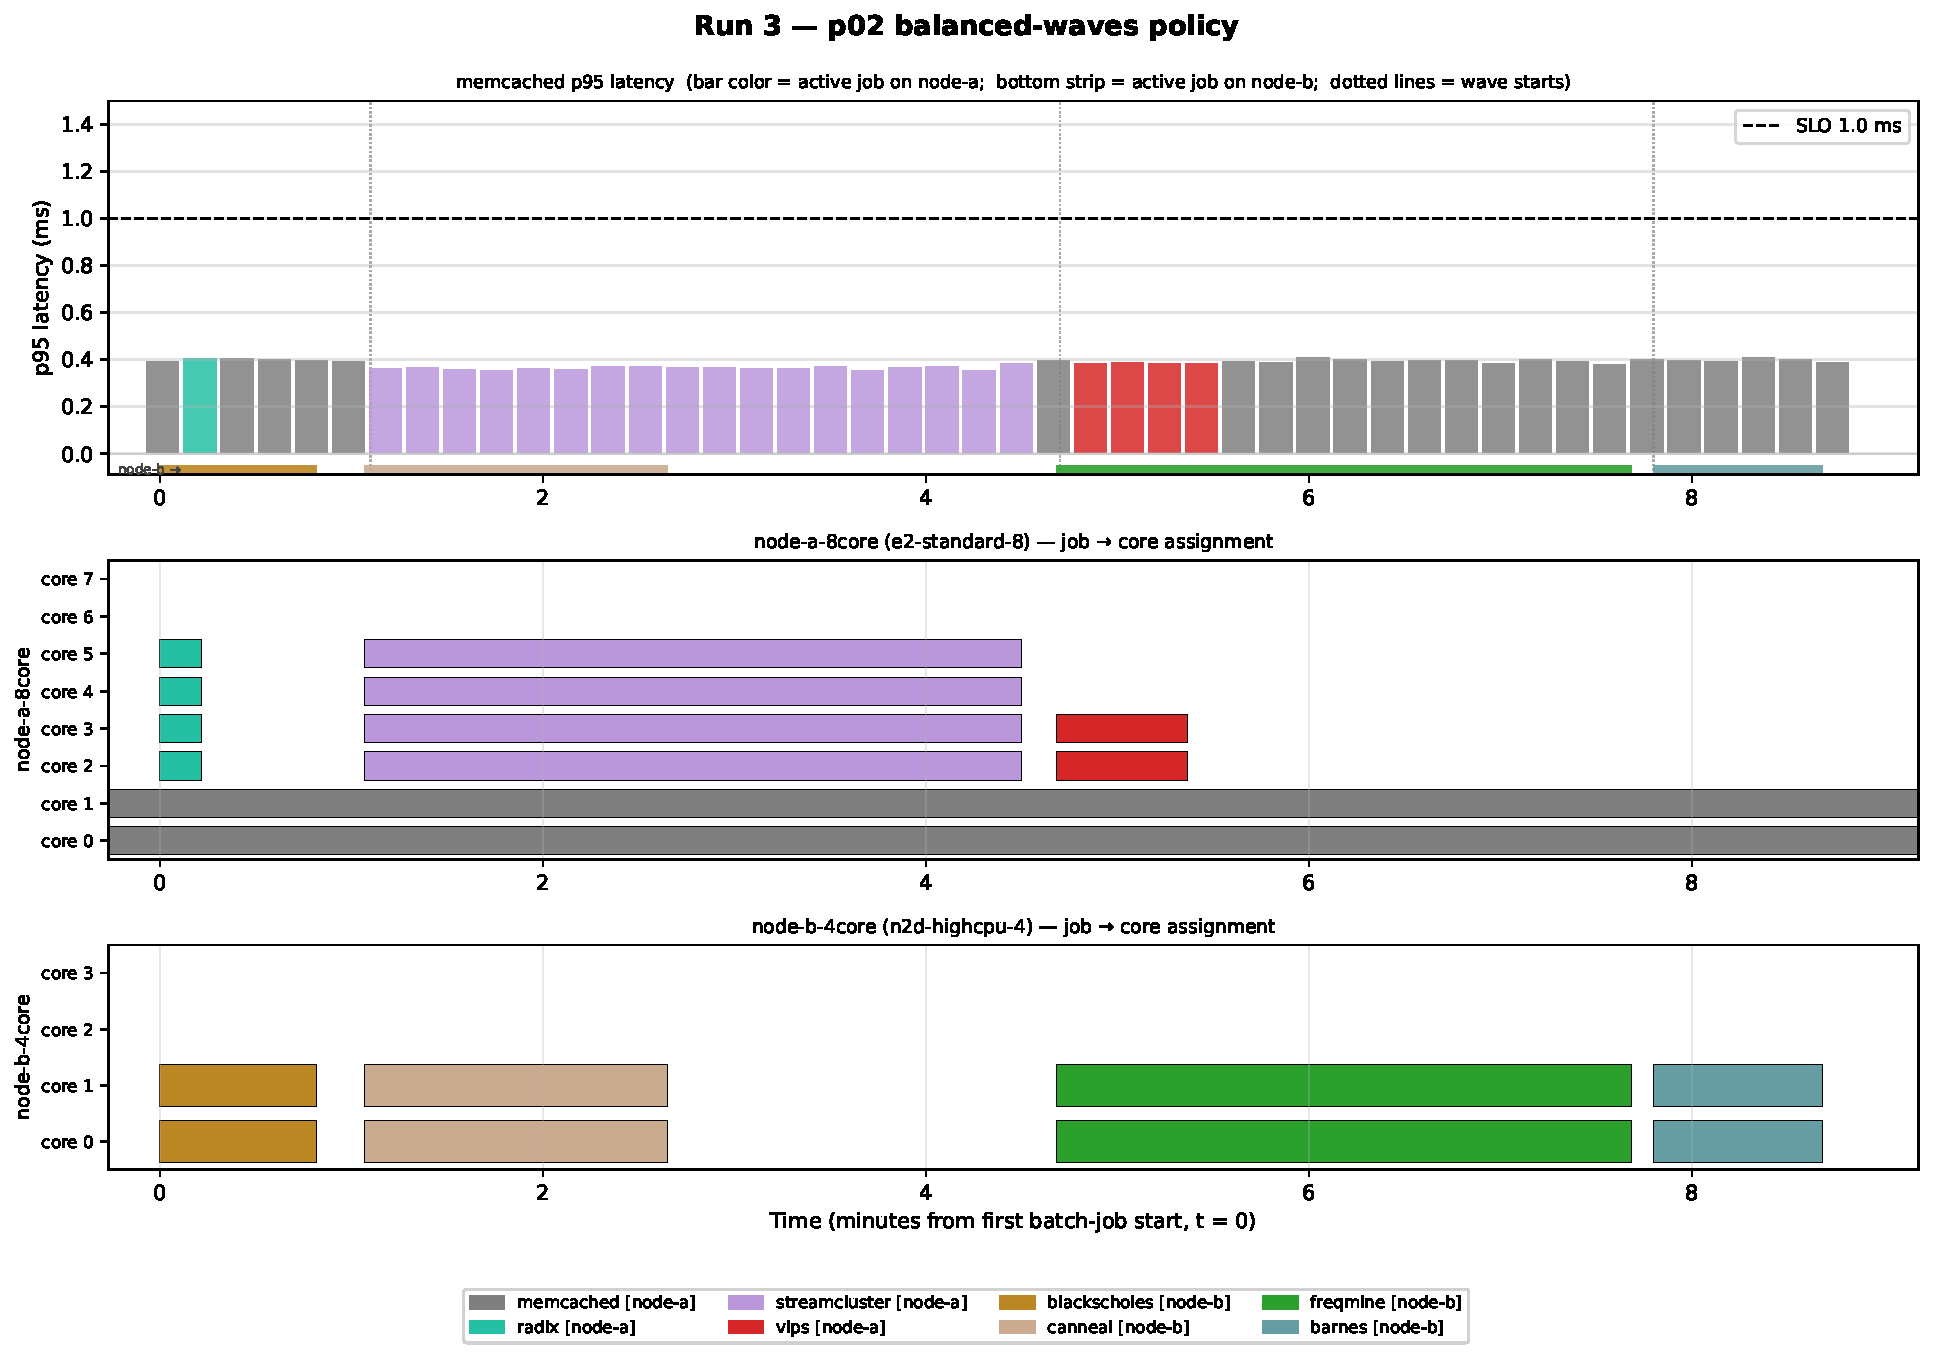
\includegraphics[width=\linewidth]{plots/part3a_run3.pdf}
  \caption{Run~3 – p95 latency and job placement (makespan 520\,s,
    SLO violations 0/46).  Run~3 is $\approx 30$\,s slower than runs~1--2,
    driven mainly by \texttt{streamcluster} (205\,s vs 193–197\,s) and
    \texttt{freqmine} (179\,s vs 165–171\,s), likely due to transient
    background load on the shared cloud infrastructure.}
  \label{fig:p3_run3}
\end{figure}

% ────────────────────────────────────────────────────────────
\subsubsection*{B. [17 points] Policy description and justification}
% ────────────────────────────────────────────────────────────

\paragraph{Which node does memcached run on?}

\textbf{Answer:} \texttt{node-a-8core} (e2-standard-8, 8 vCPUs, 32\,GB RAM).

Memcached is latency-critical and sensitive to LLC evictions (observed in
Part~1).  The e2-standard-8 VM provides a larger physical LLC, higher memory
bandwidth, and 8 vCPUs, giving memcached ample headroom.
We configure it with \textbf{2 software threads} (\texttt{-t~2}), matching its
resource request of 2~vCPUs, so the OS scheduler keeps it on dedicated cores
and batch jobs cannot fully preempt it.

\paragraph{Which node does each of the 7 batch jobs run on?}

\textbf{Answer:}
\begin{itemize}
  \item \texttt{node-a-8core}: \texttt{radix} (4\,t), \texttt{streamcluster} (4\,t), \texttt{vips} (2\,t).
  \item \texttt{node-b-4core}: \texttt{blackscholes} (2\,t), \texttt{canneal} (2\,t), \texttt{freqmine} (2\,t), \texttt{barnes} (2\,t).
\end{itemize}

\textbf{Why:}
Jobs are split to balance throughput against memcached SLO risk.
\texttt{radix} is the strongest scaler ($E(8)=0.785$) and the fastest job
(${\approx}12$\,s), so it benefits most from the faster e2-standard-8 cores
and finishes before causing any sustained LLC pressure.
\texttt{streamcluster} ($E(8)=0.581$) and \texttt{vips} ($E(8)=0.489$)
show moderate LLC interference in Part~2a but at 4 and 2 threads
respectively the per-thread cache footprint remains manageable.
The four jobs on \texttt{node-b-4core}
(\texttt{blackscholes}, \texttt{canneal}, \texttt{freqmine}, \texttt{barnes})
were the heaviest LLC and memory-bandwidth consumers in Part~2a; isolating
them on a separate node is the primary mechanism that keeps memcached's
p95 well below 1\,ms.

\paragraph{Which jobs run concurrently / are co-located?}

\textbf{Answer:}
The policy uses four sequential \emph{waves}; within each wave the assigned
jobs start simultaneously on their respective nodes:

\begin{enumerate}
  \item Wave~1: \texttt{radix} (node-a) $\|$ \texttt{blackscholes} (node-b)
  \item Wave~2: \texttt{streamcluster} (node-a) $\|$ \texttt{canneal} (node-b)
  \item Wave~3: \texttt{vips} (node-a) $\|$ \texttt{freqmine} (node-b)
  \item Wave~4: \texttt{barnes} (node-b) alone
\end{enumerate}

Jobs within a wave run at the same time but on \emph{different} physical
nodes, so there is no intra-node resource contention between batch jobs.
Memcached co-exists with the active node-a batch job on every wave.

\paragraph{In which order did you run the 7 batch jobs?}

\textbf{Order (node-a):} \texttt{radix} $\to$ \texttt{streamcluster} $\to$ \texttt{vips}

\textbf{Order (node-b):} \texttt{blackscholes} $\to$ \texttt{canneal} $\to$ \texttt{freqmine} $\to$ \texttt{barnes}

\textbf{Why:}
On node-a, \texttt{radix} goes first because it completes in ${\approx}12$\,s
and has the best scaling efficiency; it clears the node almost instantly for
\texttt{streamcluster}, which is the longest node-a job and therefore
should run as early as possible to minimise the overall critical path.
\texttt{vips} is placed last because it is short and can absorb any timing
slack without delaying the final wave.
On node-b, the order pairs shorter jobs with longer node-a partners to
maximise cross-node utilisation: \texttt{blackscholes} ($47$\,s) with
\texttt{radix} ($12$\,s), \texttt{canneal} ($95$\,s) with
\texttt{streamcluster} ($198$\,s), and \texttt{freqmine} ($172$\,s) with
\texttt{vips} ($42$\,s).

\paragraph{How many threads have you used for each of the 7 batch jobs?}

\textbf{Answer:}
\begin{itemize}
  \item \texttt{radix}: 4\,t — strong scaler ($E(8)=0.785$); 4 threads
    leave 4 vCPUs free for memcached on node-a.
  \item \texttt{streamcluster}: 4\,t — moderate scaler ($E(8)=0.581$);
    same core-budget reasoning.
  \item \texttt{vips}: 2\,t — weak scaler ($E(8)=0.489$); negligible
    throughput gain above 2 threads, and Part~2a showed increasing L1I
    interference with more threads.
  \item \texttt{blackscholes}: 2\,t — weak scaler ($E(8)=0.382$);
    diminishing returns above 2 threads make more threads wasteful.
  \item \texttt{canneal}: 2\,t — weakest scaler ($E(8)=0.369$);
    coherence bottleneck limits parallel benefit at any thread count.
  \item \texttt{freqmine}: 2\,t — moderate scaler ($E(8)=0.619$); using
    more threads on node-b-4core (4 vCPU) would leave no slack for OS
    overhead, risking OOM (as observed in p04 screening).
  \item \texttt{barnes}: 2\,t — moderate scaler ($E(8)=0.631$); same
    reasoning as \texttt{freqmine}.
\end{itemize}

Capping all node-b jobs at 2 threads keeps the total CPU request at
$2 \times 900$\,m $= 1.8$\,vCPU per job, comfortably below the 4-vCPU
limit of node-b-4core.

\paragraph{Which files did you modify or add, and which Kubernetes features
did you use?}

\textbf{Answer:}
\begin{itemize}
  \item \textbf{Added} \texttt{run\_part3a.py} — automation script that
    reads a policy from \texttt{part3\_policies.json}, launches memcached
    and batch jobs via \texttt{kubectl apply}, and polls for wave completion
    before advancing.
  \item \textbf{Added} \texttt{part3\_policies.json} — JSON policy library
    defining node assignment, thread count, and wave order for all 5
    candidate policies.
  \item \textbf{Generated on-the-fly} — Kubernetes Job manifests (one per
    batch job) with \texttt{nodeSelector} and \texttt{resources.requests}.
  \item \textbf{Modified} \texttt{memcache-t1-cpuset.yaml} — updated to
    target node-a via \texttt{nodeSelector} and run with 2 memcached
    threads.
\end{itemize}

\textbf{Kubernetes features used:}
\begin{itemize}
  \item \texttt{nodeSelector} (label \texttt{cca-project-nodetype}) — pins
    each Job pod and the memcached Pod to the correct node.
  \item \texttt{resources.requests} — declares CPU and memory requirements
    so the Kubernetes scheduler can enforce admission control and avoid
    over-commitment.
  \item \texttt{batch/v1 Jobs} with \texttt{backoffLimit: 0} — batch
    semantics with immediate failure propagation.
  \item \texttt{NodePort Service} — exposes memcached on a predictable
    port for the mcperf clients outside the cluster.
\end{itemize}

\paragraph{Design choices, trade-offs, and comparison to the second-best
policy}

\textbf{Answer:}

\textbf{Selected policy — p02\_balanced\_waves.}
The design principle is \emph{wave scheduling with strict cross-node
isolation}: each wave dispatches exactly one batch job per node and the
scheduler blocks until every job in the wave completes before launching
the next wave.
This gives two guarantees by construction: (i) no two batch jobs ever
share the same node, eliminating intra-node cache and memory-bandwidth
contention; (ii) both nodes are always productive during a wave, maximising
resource utilisation.

The policy achieves a mean makespan of $499.7 \pm 14.4$\,s with
\textbf{0\% SLO violations} across all three runs.
The coefficient of variation of 2.9\% confirms stable, reproducible
performance.

\textbf{Resource utilisation analysis.}
Table~\ref{tab:utilisation} quantifies core utilisation per node over the
mean makespan of 499.7\,s (using run~1 timings as representative).
Node-a batch utilisation counts only the 6 non-memcached cores (cores~2–7);
node-b counts all 4 cores.

\begin{table}[h]
\centering
\caption{Cluster resource utilisation — run~1 (makespan 489\,s).
  Node-a figures exclude the 2 cores reserved for memcached.}
\label{tab:utilisation}
\begin{tabular}{llrrr}
\toprule
\textbf{Wave} & \textbf{Duration [s]} &
\textbf{node-a batch cores used} &
\textbf{node-b cores used} \\
\midrule
1 (radix $\|$ blackscholes)         & 47  & 4/6 for 13\,s, then 0/6 & 2/4 \\
2 (streamcluster $\|$ canneal)      & 200 & 4/6                      & 2/4 for 95\,s, then 0/4 \\
3 (vips $\|$ freqmine)              & 172 & 2/6 for 42\,s, then 0/6 & 2/4 \\
4 (barnes only)                     & 53  & 0/6 (node-a idle)        & 2/4 \\
\midrule
\textbf{Overall (core-seconds)}     & 489 &
  908 / 2934 = \textbf{30.9\%} &
  720 / 1956 = \textbf{36.8\%} \\
\bottomrule
\end{tabular}
\end{table}

The overall batch core utilisation is 30.9\% on node-a and 36.8\% on
node-b, reflecting two structural inefficiencies of the wave-barrier
design: (i) within a wave the faster job leaves its node idle while
waiting for the slower partner; (ii) wave~4 has \textbf{node-a completely
idle} (only memcached running) because there is no eighth batch job
paired with \texttt{barnes}.

\textbf{Known weakness — wave-barrier idle time.}
The largest intra-wave gap occurs in wave~2: \texttt{streamcluster} takes
${\approx}200$\,s while \texttt{canneal} takes only ${\approx}95$\,s,
leaving node-b idle for ${\approx}105$\,s.
This is visible in Figures~\ref{fig:p3_run1}–\ref{fig:p3_run3} as the
gap in the node-b Gantt and as the grey region in the node-b strip of the
p95 chart between $t \approx 1.6$ and $4.3$\,min.
A per-node non-blocking scheduler — one that immediately dispatches the
next node-b job without waiting for node-a — could recover these idle
seconds, but would require live SLO monitoring to remain safe.
We deliberately avoided this complexity in the hand-crafted design to
guarantee predictable, verifiable SLO compliance.

\textbf{Second-best candidate — p01\_conservative\_isolation.}
This policy assigned \emph{five LLC-heavy or longer jobs} to node-b
(\texttt{canneal}, \texttt{blackscholes}, \texttt{vips},
\texttt{freqmine}, \texttt{barnes}) and routed only \texttt{radix} and
\texttt{streamcluster} to node-a — a stricter isolation strategy.
In its single screening run it recorded a makespan of \textbf{679\,s},
39\% longer than p02.
The root cause is that node-a became idle after \texttt{streamcluster}
finished at ${\approx}4.7$\,min while node-b was still processing
\texttt{freqmine} and \texttt{barnes} for another ${\approx}6.6$\,min.
The policy failed the QPS-coverage gate (no valid mcperf samples were
captured in the batch window) due to a timing issue in the measurement
setup (mcperf started before the memcached Service IP was stable), so it
was not promoted to 3 runs.
Even correcting for that measurement issue, the 37\% makespan penalty makes
p01 a clearly inferior design.

\textbf{Summary of all 5 candidates.}
Policies p03–p05 were discarded after a single run on validity grounds:
\begin{itemize}
  \item p03 (\emph{cache-aware staggered}): used 6 threads for radix on
    node-a, exceeding the node's available CPU budget after accounting for
    memcached; all pods beyond radix remained in Pending state.
  \item p04 (\emph{aggressive parallel}): used 3 threads per job on node-b;
    the combined memory footprint of multiple concurrent PARSEC jobs
    triggered OOM kills, leaving only \texttt{blackscholes} to complete.
  \item p05 (\emph{memcached-guarded}): assigned radix with 4 threads to
    node-b, fully saturating its CPU; no further jobs could be scheduled,
    and only radix completed.
\end{itemize}
These failures confirmed empirically that over-threading and concurrent
multi-job placement on the 4-core node are unsafe without explicit memory
limits, and directly motivated the conservative 2-thread-per-job cap used
in p02.
